In this section, we conduct three experiments and evaluate the performance of LRB against several bandit algorithms. Note, that at every timestep $t$, nature reveals an user $i_t$ and each algorithm suggests $d$ items to it and records all the $d$ feedbacks. The first two experiments are on simulated dataset where all our modelling assumptions hold. The third experiment is on a real-life dataset where we evaluate LRB when our modelling assumptions fail. In all our experiments users come in a Round Robin fashion over all time $[n]$. All the algorithms are averaged over $10$ independent runs.

\textbf{Contextual Algorithms:} In the contextual approach, each user has a separate version of base-bandit algorithm running independent of each other. As base-bandit algorithms we choose two versions of stochastic MAB, UCB1 and Thompson Sampling (TS), abbreviated as Contextual UCB1 (CUCB1) and Contextual TS (CTS) respectively. For UCB1, we choose the confidence interval at timestep $t$ as $c_{i_t, j}(t) = \sqrt{\frac{1.5 \log t}{N_{i_t,j}(t)}}$ for the $i_t$-th user and $j$-th item. Note, that both the vanilla UCB1 and TS is used to find the best item for each user at rank $1$, while for the remaining positions $k= 2,\dots, d$ it  suggest previously unselected items by sampling uniform randomly at every timestep $t$. 

\textbf{Matrix Completion Algorithms:} In the matrix completion approach, the algorithms try to reconstruct the user-item preference matrix $M$ from its noisy realization. We use two widely used method to reconstruct partially observed noisy matrices, linear ridge regression and non-negative matrix factorization. We term the corresponding algorithms as Linear Bandit (LinBan) and NMF Bandit (NMF-Ban) respectively. Both of these algorithms are $\epsilon$-greedy in implementation whereby they reconstruct $M$ with $\epsilon$ probability and with $1-\epsilon$ probability they behave greedily over the reconstructed matrix and suggest $d$ best item for the $i_t$-th user at every timestep $t$. LinBan uses ridge regression to reconstruct $M$ from its estimated $d$-best columns while NMF-Ban uses matrix factorization to estimate the $U$ and $V$ matrix and reconstruct $M$ from its noisy realization.

\textbf{Personalized Ranking Algorithms:} In this approach, we evaluate our proposed algorithm Latent Ranking Bandit (LRB) by using two different types of base-bandits, EXP3 and UCB1 as column MABs. We term them as LREXP3 and LRUCB1 respectively. For LREXP3 we set the column exploration parameter $\gamma_k = \sqrt{\frac{L \log L}{n}}, \forall \text{ MAB}_k(n), k = 1,\dots, d$ and for LRUCB1 we use  a confidence interval of $c_{k, j}(t) = \sqrt{\frac{1.5 \log t}{N_{k,j}(t)}}$ for the $k$-th column MAB and $j$-th item.

\textbf{Experiment 1:} This experiment is conducted to test the performance of LRB over  small number of users and items. This simulated testbed consist of $500$ users, $50$ items and rank$(M) = 2$. The vectors spanning $U$ and $V$, generating the user-item preference matrix $M$ is shown Figure \ref{fig:1}. The users are divided into a $70:30$ split such that $70\%$ of users prefer item $j^*_1$ and $30\%$ users prefer item  $j^*_2$. The item hott-topics are $V(1:) = (0,1)$ and $V(2,:) = (1, 0)$ while remaining $70\%$ of items has feature $V(\ell_{j'},:) = (0.45, 0.55)$ and the rest have $V(\ell_{j}) = (0.55, 0.45)$. We create the user feature matrix $U$ similarly having a $70:30$ split such that $U(1,:) = (0,1)$, $U(2,:) = (1,0)$ and the remaining $70\%$ users having $U(i,:) = (0,0.8)$ and $30\%$ users having $U(i',:) = (0.7,0)$. The resultant matrix $M =UV^{\intercal}$ is such that algorithms that quickly find the easily identifiable hott-topics perform very well. From Figure \ref{fig:2} we can clearly see that both LREXP3 and LRUCB1 outperforms all the other algorithms. Their regret curve flattens, indicating that they have learned the best items for each user.  NMF-Ban and LinBan has nearly similar performance as both of these algorithms fail to get a reasonable approximation of $M$ although they perform better than CUCB1. Contextual algorithm CUCB1 performs poorly as the number of items per user is too large and the gaps are also small. Although CTS performs well in this small testbed, its performance eventually degrades for larger environments. 


\begin{figure}[!th]
\centering
\begin{tabular}{cc}
\setlength{\tabcolsep}{0.1pt}
\subfigure[0.25\textwidth][Expt-$1$: $500$ Users, $50$ items, Rank $2$, User and Item vectors]
    %with $r_{i_{{i}\neq {*}}}=0.07$ and $r^{*}=0.1$
    {
    		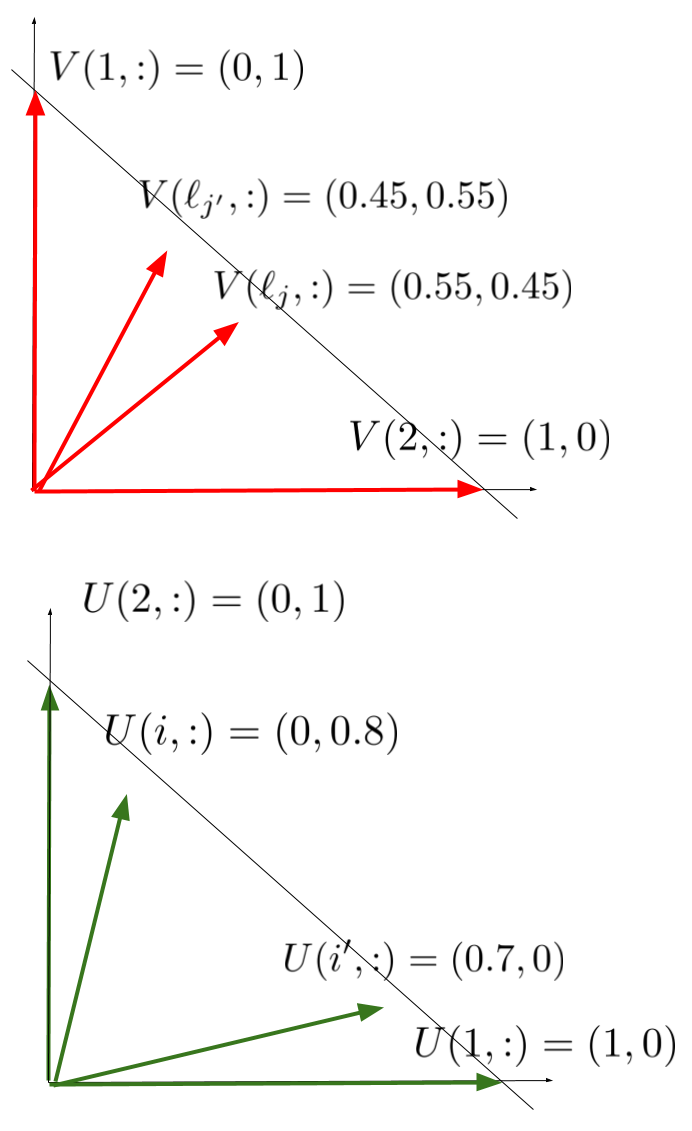
\includegraphics[scale=0.11]{img/rank2_vec.png}
  		\label{fig:1}
    }
    &
    \subfigure[0.25\textwidth][Expt-$1$: Cumulative regret of different algorithms]
    %with $r_{i_{{i}\neq {*}}}=0.07$ and $r^{*}=0.1$
    {
    		\pgfplotsset{
		tick label style={font=\Large},
		label style={font=\Large},
		legend style={font=\Large},
		ylabel style={yshift=5pt},
		%legend style={legendshift=32pt},
		}
        \begin{tikzpicture}[scale=0.4]
      	\begin{axis}[
		xlabel={timestep},
		ylabel={Cumulative Regret},
		grid=major,
        %clip mode=individual,grid,grid style={gray!30},
        clip=true,
        %clip mode=individual,grid,grid style={gray!30},
        cycle list name=exotic,
  		legend style={at={(0.5,1.4)},anchor=north, legend columns=3} ]
      	% UCB
		\addplot table{results/NewExpt1/Expt1/comp_subsampled_CTS0RR1S.txt};
		\addplot table{results/NewExpt1/Expt1/comp_subsampled_LRUCB0RR1S.txt};
		\addplot table{results/NewExpt1/Expt1/comp_subsampled_LREXP30RR1S.txt};
		\addplot table{results/NewExpt1/Expt1/comp_subsampled_NMF0RR1S.txt};
		\addplot table{results/NewExpt1/Expt1/comp_subsampled_LinBan0RR1S.txt};
		\addplot table{results/NewExpt1/Expt1/comp_subsampled_CUCB10RR1S.txt};
		\legend{CTS, LRUCB1, LREXP3, NMF-Ban, LinBan, CUCB1} 
      	\end{axis}
      	\end{tikzpicture}
  		\label{fig:2}
    }
    \\
    \subfigure[0.25\textwidth][Expt-$2$: $1500$ Users, $100$ items, Rank $3$, User and Item vectors]
    %with $r_{i_{{i}\neq {*}}}=0.07$ and $r^{*}=0.1$
    {
    		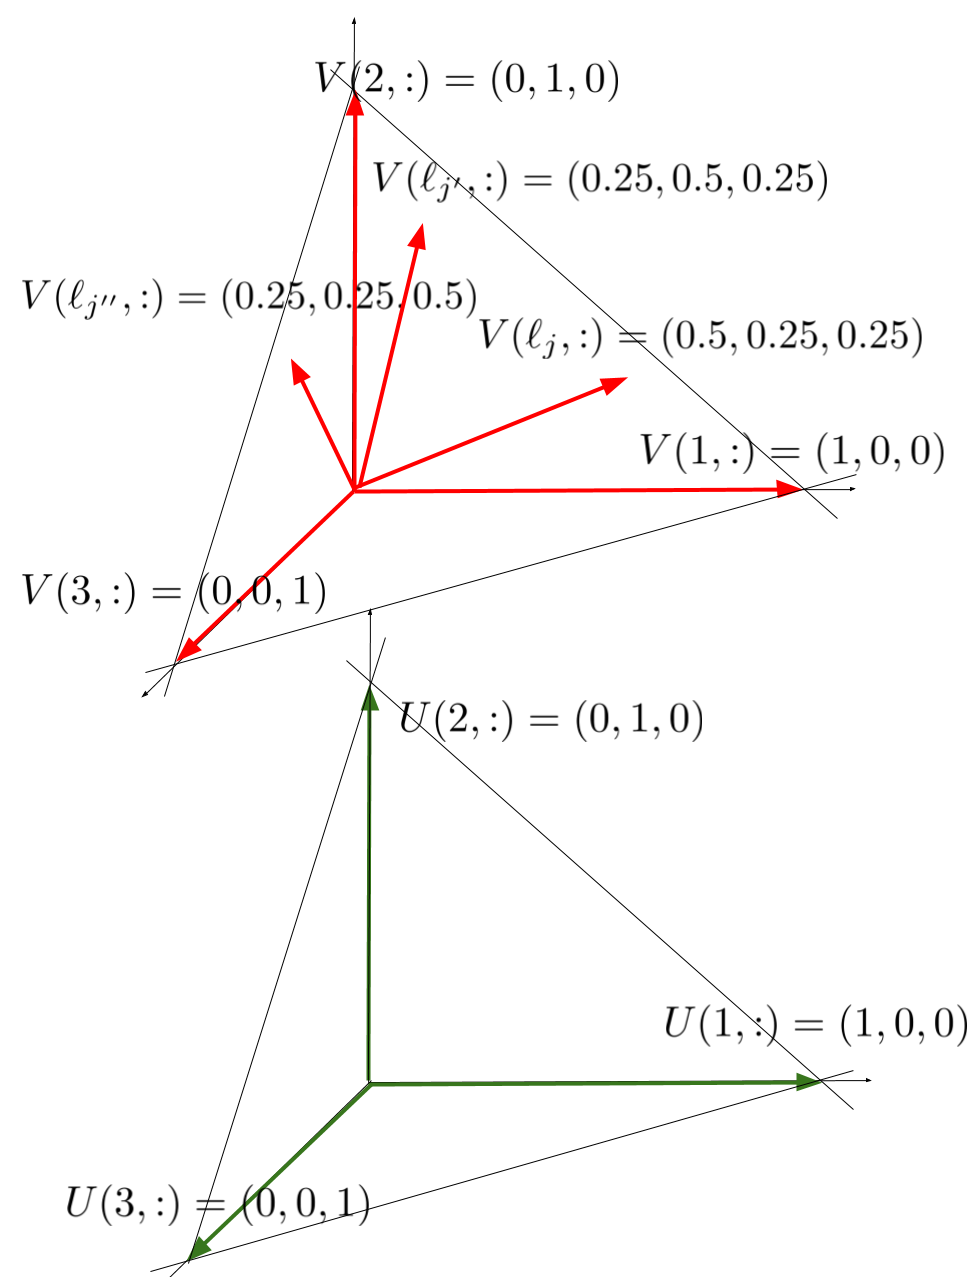
\includegraphics[scale=0.11]{img/rank3_vec.png}
  		\label{fig:3}
    }
    &
    \subfigure[0.25\textwidth][Expt-$2$: Cumulative regret of different algorithms]
    %with $r_{i_{{i}\neq {*}}}=0.07$ and $r^{*}=0.1$
    {
    		\pgfplotsset{
		tick label style={font=\Large},
		label style={font=\Large},
		legend style={font=\Large},
		ylabel style={yshift=5pt},
		%legend style={legendshift=32pt},
		}
        \begin{tikzpicture}[scale=0.4]
      	\begin{axis}[
		xlabel={timestep},
		ylabel={Cumulative Regret},
		grid=major,
        %clip mode=individual,grid,grid style={gray!30},
        clip=true,
        %clip mode=individual,grid,grid style={gray!30},
        cycle list name=exotic,
  		legend style={at={(0.5,1.4)},anchor=north, legend columns=3} ]
      	% UCB
		\addplot table{results/NewExpt1/Expt2/comp_subsampled_CTS0RR1S.txt};
		\addplot table{results/NewExpt1/Expt2/comp_subsampled_LRUCB0RR1S.txt};
		\addplot table{results/NewExpt1/Expt2/comp_subsampled_LREXP30RR1S.txt};
		\addplot table{results/NewExpt1/Expt2/comp_subsampled_NMF0RR1S.txt};
		\addplot table{results/NewExpt1/Expt2/comp_subsampled_LinBan0RR1S.txt};
		\addplot table{results/NewExpt1/Expt2/comp_subsampled_CUCB10RR1S.txt};
		\legend{CTS, LRUCB1, LREXP3, NMF-Ban, LinBan, CUCB1} 
      	\end{axis}
      	\end{tikzpicture}
  		\label{fig:4}
    }
    \end{tabular}
    \caption{A comparison of the cumulative regret incurred by the various bandit algorithms. }
    \label{fig:karmed1}
    \vspace*{-1em}
\end{figure}

\textbf{Experiment 2:} We conduct the second experiment on a larger simulated database of $1500$ users, $100$ items and rank$(M)=3$. The vectors spanning $U$ and $V$, generating the user-item preference matrix $M$ is shown Figure \ref{fig:3}. The users are divided into a $60:30:10$ split such that $60\%$ of the users prefer item $j^*_1$, $30\%$ prefer $j^*_2$ and $10\%$ prefer $j_3^*$.  Here, hott-topics are $V(1,:) = (1,0,0)$, $V(2,:) = (0,1, 0)$ and $V(3,:) = (0,0,1)$. The remaining $60\%$ of items have feature  $V(\ell_{j},:) = (0.5, 0.25,0.25)$, $30\%$ have $V(\ell_{j'}) = (0.25, 0.5, 0.25)$ and rest have $V(\ell_{j''}) = (0.25, 0.25, 0.5)$. We create the user feature matrix $U$ similarly having a $60:30:10$ split and the vectors spanning $U$ are only of the type that spans the simplex, i.e $U(i,:)=(1,0,0)$, $U(i',:)=(1,0,0)$ and $U(i^{''},:)=(1,0,0)$. Again, the resultant matrix $M =UV^{\intercal}$ is such that algorithms that quickly spot the easily identifiable hott-topics outperform others. From Figure \ref{fig:4} we can see that both LREXP3 and LRUCB1 again outperforms all the other algorithms. Their regret curve flattens much before all the other algorithms indicating that they have learned the best items for each user. The matrix completion algorithms NMF-Ban and LinBan fail to get a reasonable approximation of $M$ and perform poorly. Also, we see that both the contextual algorithms CUCB1 and CTS perform poorly as the number of users and the number of items per user is too large and the independent base-bandits are not sharing information between themselves. In both the simulated datasets, we see that stochastic column MAB (UCB1) is outperforming adversarial column MAB (EXP3) as the user preference over the best item is not changing over time. This has also been observed by \citet{radlinski2008learning}.

%which stems from the fact that all the user, 

\textbf{Experiment 3:} We conduct the third experiment to test the performance of LRB when our modelling assumptions are violated. We use the Jester dataset \citep{goldberg2001eigentaste} which consist of over 4.1 million continuous ratings of 100 jokes from 73,421 users collected over 5 years. We sample randomly around 2000 users from this dataset and use singular value decomposition (SVD) to obtain a rank $2$ approximation of this user-joke rating matrix $M$. The rank $2$ approximation of $M$ of  is shown in Figure \ref{fig:5}, where we can clearly see the red stripes spanning the matrix indicating the low-rank structure of $M$. Furthermore, in this experiment we assume that the noise is independent Bernoulli over the entries of $M$ and hence this experiment deviates from our modeling assumptions. From \ref{fig:6} again we see that LREXP3 outperforms other algorithms. The regret curve of LRUCB1 does not flatten out which we attribute to the fact that LRUCB1 uses too large a confidence interval. The contextual and matrix completion algorithms perform significantly worse in this large testbed.



%[[1104, 99], [896, 93],[0,0][0,0]}

\begin{figure}[!th]
\centering
\begin{tabular}{cc}
\setlength{\tabcolsep}{0.1pt}
\subfigure[0.25\textwidth][Expt-$3$: $2000$ Users, $100$ items, Rank $2$ approximation of Jester Dataset]
    %with $r_{i_{{i}\neq {*}}}=0.07$ and $r^{*}=0.1$
    {
    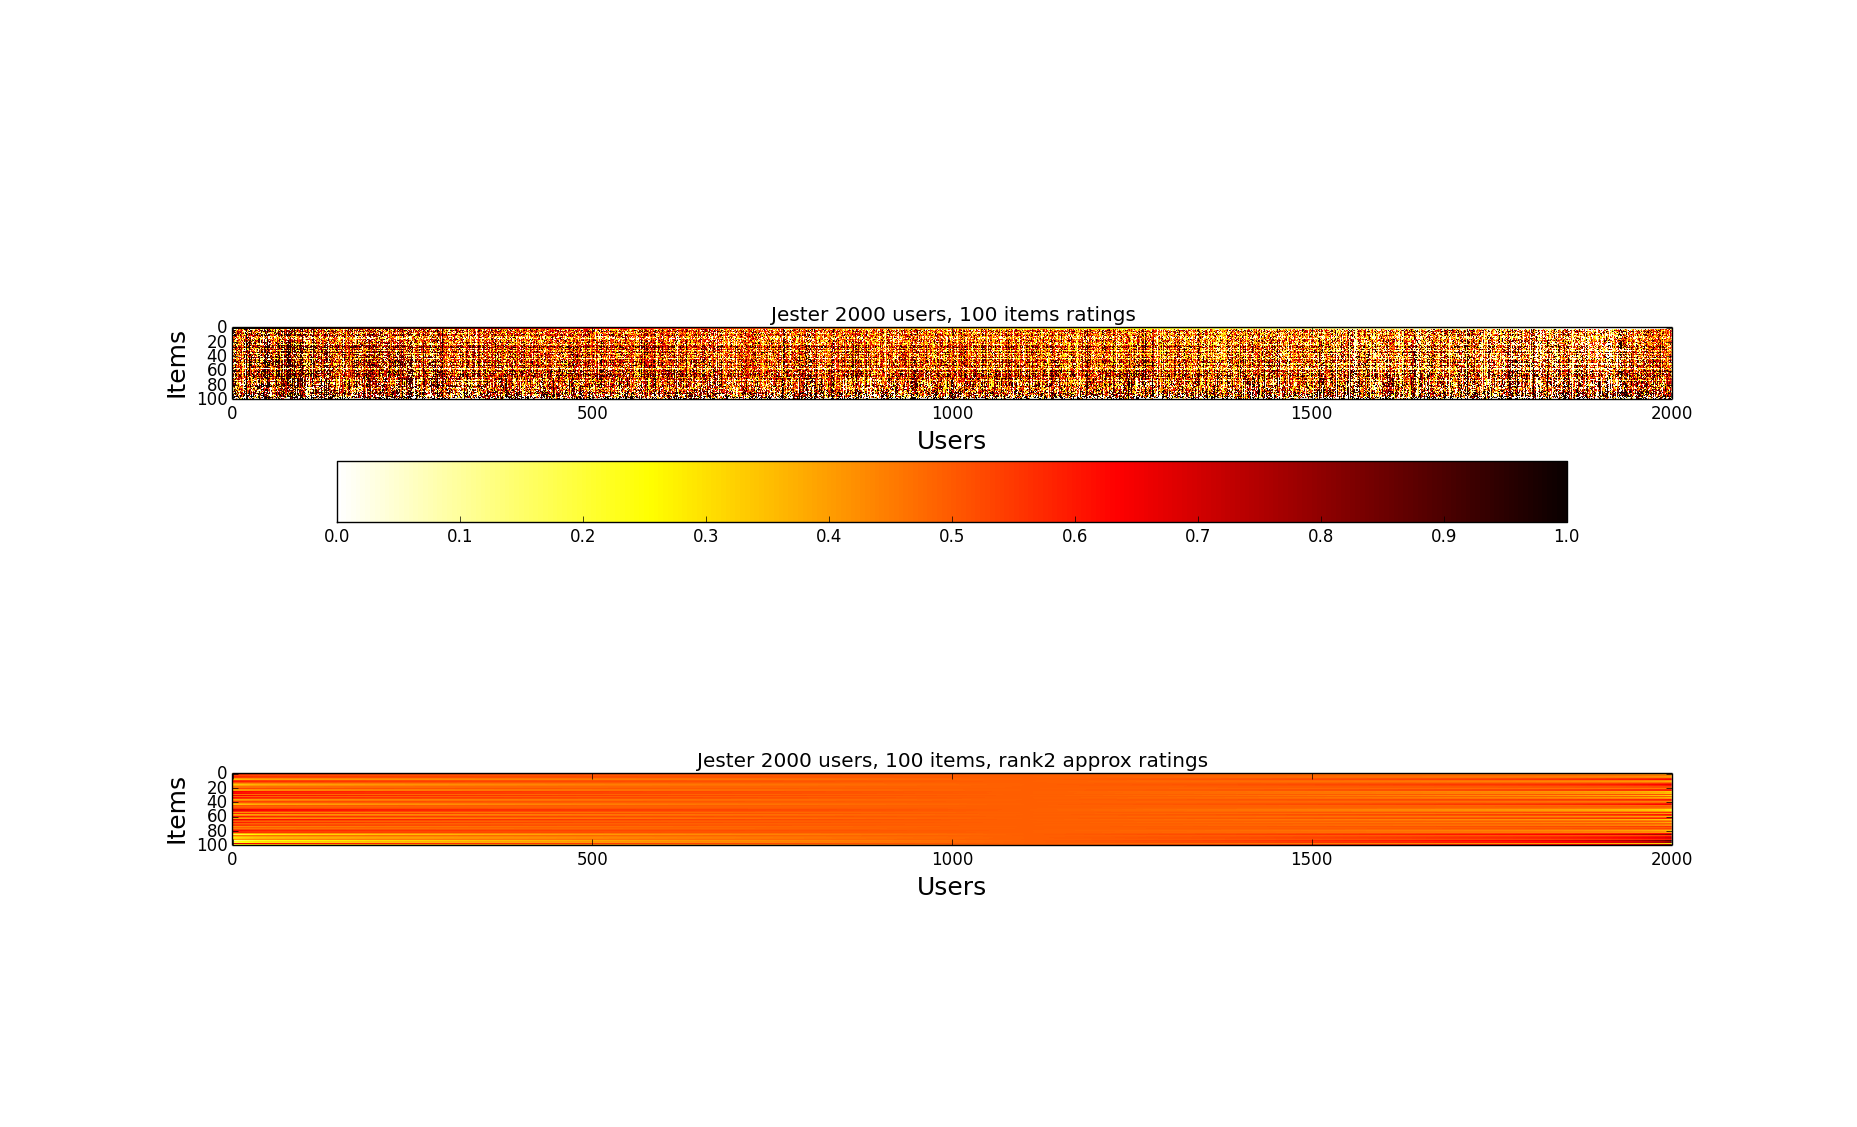
\includegraphics[scale=0.08]{img/jester_rank2.png}
    	\label{fig:5}
    }
    &
\subfigure[0.25\textwidth][Expt-$3$: Cumulative regret of different algorithms]
    %with $r_{i_{{i}\neq {*}}}=0.07$ and $r^{*}=0.1$
    {
    		\pgfplotsset{
		tick label style={font=\Large},
		label style={font=\Large},
		legend style={font=\Large},
		ylabel style={yshift=5pt},
		%legend style={legendshift=32pt},
		}
        \begin{tikzpicture}[scale=0.4]
      	\begin{axis}[
		xlabel={timestep},
		ylabel={Cumulative Regret},
		grid=major,
        %clip mode=individual,grid,grid style={gray!30},
        clip=true,
        cycle list name=exotic,
        %clip mode=individual,grid,grid style={gray!30},
  		legend style={at={(0.5,1.4)},anchor=north, legend columns=3} ]
      	% UCB
		
		\addplot table{results/NewExpt1/Expt3/comp_subsampled_CTS0RR1S.txt};
		\addplot table{results/NewExpt1/Expt3/comp_subsampled_LRUCB0RR1S.txt};
		\addplot table{results/NewExpt1/Expt3/comp_subsampled_LREXP30RR1S.txt};
		\addplot table{results/NewExpt1/Expt3/comp_subsampled_NMF0RR1S.txt};
		\addplot table{results/NewExpt1/Expt3/comp_subsampled_LinBan0RR1S.txt};
		\addplot table{results/NewExpt1/Expt3/comp_subsampled_CUCB10RR1S.txt};
		\legend{CTS, LRUCB1, LREXP3, NMF-Ban, LinBan, CUCB1} 
      	\end{axis}
      	\end{tikzpicture}
  		\label{fig:6}
    }
 \end{tabular}
    \caption{A comparison of the cumulative regret in Jester Dataset }
    \label{fig:karmed}
    \vspace*{-1em}
\end{figure}